\documentclass[submit]{../harvardml}


\course{CS1810-S25}
\assignment{Assignment \#1}
\duedate{11:59pm ET, February 14, 2025} 

\usepackage[OT1]{fontenc}
\usepackage[colorlinks,citecolor=blue,urlcolor=blue]{hyperref}
\usepackage{graphicx}
\usepackage{caption}
\usepackage{enumitem}
\usepackage{soul}
\usepackage{amsmath}
\usepackage{amssymb}
\usepackage{color}
\usepackage{todonotes}
\usepackage{listings}
\usepackage{../common}
\usepackage{framed}
\usepackage{float}
\usepackage{ifthen}
\usepackage{bm}
\usepackage[breakable]{tcolorbox}
\lstdefinestyle{mystyle}{
    backgroundcolor=\color{white},    % set background color
    commentstyle=\color{green!50!black},
    keywordstyle=\color{blue},
    numberstyle=\tiny\color{gray},
    stringstyle=\color{red},
    basicstyle=\ttfamily\footnotesize, % use a monospaced font
    breakatwhitespace=false,           % automatic breaks
    breaklines=true,                   % break long lines
    captionpos=b,                      % position of the caption
    keepspaces=true,                   % keep spaces in text
    numbers=left,                      % line numbers on the left
    numbersep=5pt,                     % spacing between numbers and code
    showspaces=false,
    showstringspaces=false,
    showtabs=false,
    tabsize=4,
}

\usepackage[mmddyyyy,hhmmss]{datetime}

\definecolor{verbgray}{gray}{0.9}

\lstnewenvironment{csv}{
  \lstset{backgroundcolor=\color{verbgray},
  frame=single,
  framerule=0pt,
  basicstyle=\ttfamily,
  columns=fullflexible}}{}

 \DeclareMathOperator*{\limover}{\overline{lim}}

%%%%%%%%%%%%%%%%%%%%%%%%%%%%%%%%%%
%% Solution environment
\usepackage{xcolor}
\usepackage{comment}
\newenvironment{solution}
  {\color{blue}\section*{Solution}}
{}
%%%%%%%%%%%%%%%%%%%%%%%%%%%%%%%%%%



\begin{document}
\begin{center}
  {\Large Homework 1: Regression}\\
\end{center}

\subsection*{Introduction}
This homework is on different three different forms of regression:
kernelized regression, nearest neighbors regression, and linear
regression.  We will discuss implementation and examine their
tradeoffs by implementing them on the same dataset, which consists of
temperature over the past 800,000 years taken from ice core samples.

The folder \verb|data| contains the data you will use for this
problem. There are two files:
\begin{itemize}
  \item \verb|earth_temperature_sampled_train.csv|
  \item \verb|earth_temperature_sampled_test.csv|
\end{itemize}

Each has two columns.  The first column is the age of the ice core
sample.  The second column is the approximate difference in a year's temperature (K)
from the average temperature of the 1,000 years preceding it. The temperatures were retrieved from ice cores in
Antarctica (Jouzel et al. 2007)\footnote{Retrieved from
  \url{https://www.ncei.noaa.gov/pub/data/paleo/icecore/antarctica/epica_domec/edc3deuttemp2007.txt}

  Jouzel, J., Masson-Delmotte, V., Cattani, O., Dreyfus, G., Falourd,
  S., Hoffmann, G., … Wolff, E. W. (2007). Orbital and Millennial
  Antarctic Climate Variability over the Past 800,000 Years.
  \emph{Science, 317}(5839), 793–796. doi:10.1126/science.1141038}.

The following is a snippet of the data file:

\begin{csv}
  # Age, Temperature
  399946,0.51
  409980,1.57
\end{csv}

\noindent And this is a visualization of the full dataset:
\begin{center}
  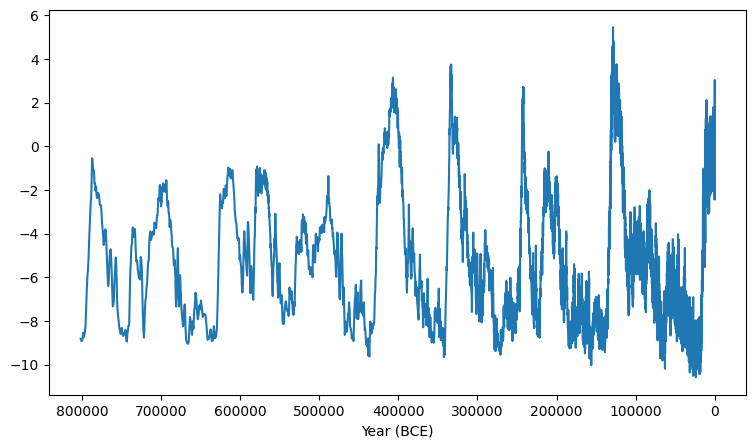
\includegraphics[width=.8\textwidth]{img_input/sample_graph}
\end{center}
\noindent


\textbf{Due to the large magnitude of the years, we will work in terms
  of thousands of years BCE in these problems.} This is taken care of
for you in the provided notebook.






\subsection*{Resources and Submission Instructions}
If you find that you are having trouble with the first couple
problems, we recommend going over the fundamentals of linear algebra
and matrix calculus (see links on website).  The relevant parts of the
\href{https://github.com/harvard-ml-courses/cs181-textbook/blob/master/Textbook.pdf}{cs181-textbook
  notes are Sections 2.1 - 2.7}.  We strongly recommend reading the
textbook before beginning the homework.

We also encourage you to first read the
\href{http://users.isr.ist.utl.pt/~wurmd/Livros/school/Bishop\%20-\%20Pattern\%20Recognition\%20And\%20Machine\%20Learning\%20-\%20Springer\%20\%202006.pdf}{Bishop
  textbook}, particularly: Section 2.3 (Properties of Gaussian
Distributions), Section 3.1 (Linear Basis Regression), and Section 3.3
(Bayesian Linear Regression). (Note that our notation is slightly
different but the underlying mathematics remains the same!).

\textbf{Please type your solutions after the corresponding problems
  using this \LaTeX\ template, and start each problem on a new page.}
You may find the following introductory resources on \LaTeX\ useful:
\href{http://www.mjdenny.com/workshops/LaTeX_Intro.pdf}{\LaTeX\ Basics}
and
\href{https://www.overleaf.com/learn/latex/Free_online_introduction_to_LaTeX_(part_1)}{\LaTeX\ tutorial
  with exercises in Overleaf}

Homeworks will be submitted through Gradescope. You will be added to
the course Gradescope once you join the course Canvas page. If you
haven't received an invitation, contact the course staff through Ed.

\textbf{Please submit the writeup PDF to the Gradescope assignment
  `HW1'.} Remember to assign pages for each question.

\textbf{Please submit your \LaTeX file and code files to the
  Gradescope assignment `HW1 - Supplemental'.} Your files should be
named in the same way as we provide them in the repository,
e.g. \texttt{hw1.pdf}, etc.

%%%%%%%%%%%%%%%%%%%%%%%%%%%%%%%%%%%%%%%%%%%%%
% Problem 1
%%%%%%%%%%%%%%%%%%%%%%%%%%%%%%%%%%%%%%%%%%%%%
\begin{problem}[kNN and Kernels, 35pts]

You will now implement two non-parametric regressions to model temperatures over time.  
% For this problem, you will use the \textbf{same dataset as in Problem 1}.

\vspace{0.5cm}
\noindent\emph{Make sure to include all required plots in your PDF. Passing all test cases does not guarantee that your solution is correct, and we encourage you to write your own. }

\begin{enumerate}
\item 
 Recall that kNN uses a predictor of the form
\[
  f(x^*) = \frac{1}{k} \sum_n y_n \mathbb{I}(x_n \texttt{ is one of k-closest to } x^*),
\]
where $\mathbb{I}$ is an indicator variable. 
\begin{enumerate}

  \item The kNN implementation \textbf{has been provided for you} in the notebook. Run the cells to plot the results for $k=\{1, 3, N-1\}$, where $N$ is the size of the dataset. Describe how the fits change with $k$. Please include your plot in your solution PDF.

  \item Now, we will evaluate the quality of each model \emph{quantitatively} by computing the error on the provided test set. Write Python code to compute test MSE for each value of $k$.  Which solution has the lowest MSE? 
  
\end{enumerate}

\item \textit{Kernel-based regression} techniques are another form of non-parametric regression. Consider a kernel-based
regressor of the form 
\begin{equation*}
  f_\tau(x^*) = \cfrac{\sum_{n} K_\tau(x_n,x^*) y_n}{\sum_n K_\tau(x_n, x^*)}
\end{equation*}
where $\mathcal{D}_\texttt{train} = \{(x_n,y_n)\}_{n = 1} ^N$ are the
training data points, and $x^*$ is the point for which you want to
make the prediction.  The kernel $K_\tau(x,x')$ is a function that
defines the similarity between two inputs $x$ and $x'$. A popular
choice of kernel is a function that decays as the distance between the
two points increases, such as
\begin{equation*}
  K_\tau(x,x') = \exp\left(-\frac{(x-x')^2}{\tau}\right)
\end{equation*}

where $\tau$ represents the square of the lengthscale (a scalar value that
dictates how quickly the kernel decays).  


\begin{enumerate}
    
  \item First, implement the \texttt{kernel\_regressor} function in the notebook, and plot your model for years in the range $800,000$ BC to $400,000$ BC at $1000$ year intervals for the following three values of $\tau$: $1, 50, 2500$. Since we're working in terms of thousands of years, this means you should plot $(x, f_\tau(x))$ for $x = 400, 401, \dots, 800$. \textbf{In no more than 10 lines}, describe how the fits change with $\tau$. Please include your plot in your solution PDF.

  \item Denote the test set as $\mathcal{D}_\texttt{test} = \{(x'_m, y'_m)\}_{m = 1} ^M$.  Write down the expression for MSE of $f_\tau$ over the test set as a function of the training set and test set. Your answer may include $\{(x'_m, y'_m)\}_{m = 1} ^M$, $\{(x_n, y_n)\}_{n = 1} ^N$, and $K_\tau$, but not $f_\tau$.

    \item Compute the MSE on the provided test set for the three values of $\tau$.  Which model yields the lowest MSE? Conceptually, why is this the case? Why would choosing $\tau$ based on $\mathcal{D}_\texttt{train}$ rather than $\mathcal{D}_\texttt{test}$ be a bad idea? 

  \item Describe the time and space complexity of both kernelized regression and kNN with respect to the size of the training set $N$.  How, if at all, does the size of the model---everything that needs to be stored to make predictions---change with the size of the training set $N$?  How, if at all, do the number of computations required to make a prediction for some input $x^*$ change with the size of the training set $N$?.
  

  \item  What is the exact form of $\lim_{\tau \to 0 }f_\tau(x^*)$?
  \end{enumerate}
\end{enumerate}
\end{problem}

\newpage
\begin{solution}


\begin{enumerate}
  \item a) 

  As $\tau$ increases, the model becomes smoother and less sensitive to noise.
  Even as  $\tau$ gets extremely large, it still is able to capture some of the patterns in the data, which is not true for kNN; kNN converges to the mean of the dataset as $k \to N$. In this case, the kernelized model converges slower. 

  \begin{figure}[h]
    \centering
    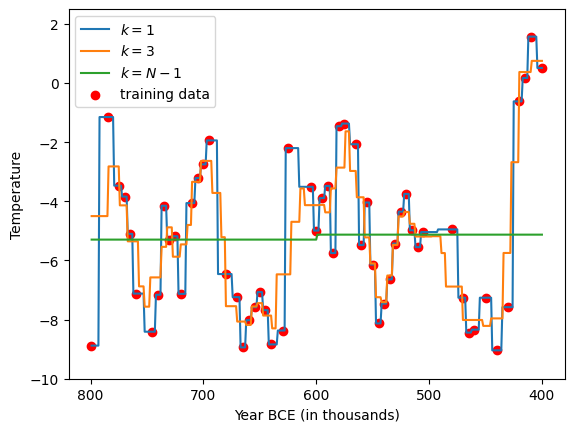
\includegraphics[width=0.5\textwidth]{img_output/p1.1a.png}
    \caption{Plot of the kNN model fits for different values of $k$.}
  \end{figure}


  \begin{figure}[h]
    \centering
    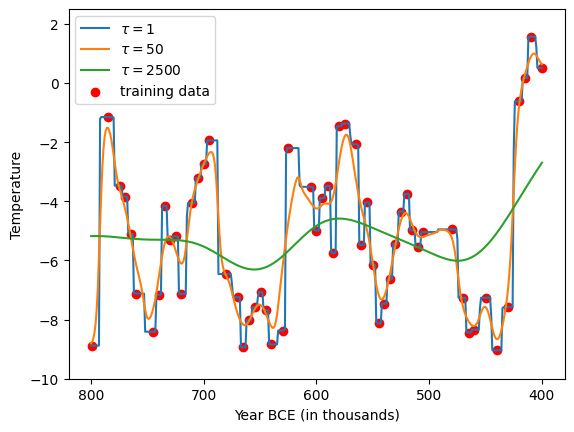
\includegraphics[width=0.5\textwidth]{img_output/p1.2a.png}
    \caption{Plot of the kernel modle fits for different values of $\tau$.}
  \end{figure}

  b)
  \begin{lstlisting}[language=Python]

    def model_mse(predictions, true):
    """
    Calculate the MSE for the given model predictions, with respect to the true values

    :param predictions: predictions given by the model
    :param true: corresponding true values
    :return: the mean squared error
    """
    return np.mean((predictions - true) ** 2)

    k_values = [1, 3, len(year_train) - 1]
for k in k_values:
    preds = predict_knn(year_test, k, year_train, temp_train)
    mse = model_mse(preds, temp_test)
    print(f"k = {k}, Test MSE = {mse}")

    \end{lstlisting}

    k = 1, Test MSE = 1.7406000000000004 \newline
    k = 3, Test MSE = 3.8907662222222212 \newline
    k = 56, Test MSE = 9.528571442602042

  
  \item 
  

  \[
\text{MSE} = \frac{1}{M} \sum_{m=1}^{M} \left( y'_m - \frac{\sum_{n=1}^{N} K_\tau(x_n, x'_m) \, y_n}{\sum_{n=1}^{N} K_\tau(x_n, x'_m)} \right)^2
\]



  \item 
  
  After computing the test set MSEs for \(\tau = 1\), \(\tau = 50\), and \(\tau = 2500\), we observed that the model with \(\tau = 50\) yields the lowest MSE.


  Conceptually, this makes sense because:
  \begin{itemize}
    \item A small \(\tau\) leads to overfitting, as the model becomes too sensitive to noise in the training data.
    \item A large \(\tau\) leads to underfitting, as the model fails to capture the underlying patterns in the data; it just fits to the average values and does not weight the data points appropriately.
  \end{itemize}

  Choosing \(\tau\) based on \(\mathcal{D}_\texttt{train}\) rather than \(\mathcal{D}_\texttt{test}\) would be a bad idea because it would lead to overfitting on the training data. The test data is very helpful because it allows us to evaluate the model based on data it hasn't seen yet, but which is still representative of the real, unerlying data-generating process. If we choose \(\tau\) based on the training data, the tau with the loweest MSE would be the smallest tau tested because it would be the closest fit to the training data, but would not generalize to unseen data. 


  \item d)
  
  Time complexity

  To determine the time complexity, we need to understand what is occuring for each data point. For each data point, we must calculate the kernel for every other data point. Thus, the time complexity is \(O(N^2)\) because for every data point n in N, we have to do N calculations.$ N \times N = N^2$. 

  Space complexity is \(O(N)\) because we need to store N data points.


  \item e)
  
   \[
    \lim_{\tau \to 0} f_\tau(x^*) = \frac{\sum_{n=1}^N \mathbb{I}\{x_n = x^*\}\, y_n}{\sum_{n=1}^N \mathbb{I}\{x_n = x^*\}},
    \]

    where \(\mathbb{I}\) is the indicator function.

      If \(x_n = x^*\), then \(K_\tau(x_n, x^*) = 1\) and all other terms are 0. Thus, the limit is equal to the value of \(y_n\) for that data point.


\end{enumerate}







\end{solution}


%%%%%%%%%%%%%%%%%%%%%%%%%%%%%%%%%%%%%%%%%%%%%
% Problem 2
%%%%%%%%%%%%%%%%%%%%%%%%%%%%%%%%%%%%%%%%%%%%%
\newpage
\begin{problem}[Deriving Linear Regression, 20pts]

We now seek to model the temperatures with a parametric method: linear regression. Before we implement anything, let's revisit the mathematical formulation of linear regression.  Specifically, the solution for the least squares linear regression  ``looks'' kind of like a ratio of covariance and
variance terms.  In this problem, we will make that connection more
explicit. \\

\noindent Suppose we have some 2-D data where each observation has the form $(x, y)$ and is independent and identically distributed according  $x \sim p(x)$, $y \sim p(y|x)$. We will consider the process of fitting these data from this distribution with the best linear model
possible, that is a linear model of the form $\hat{y} = wx$ that
minimizes the expected squared loss $E_{x,y}[ ( y - \hat{y} )^2
    ]$.\\

\noindent Note: The notation $E_{x, y}$ indicates an
expectation taken over the joint distribution $p(x,y)$. This essentially just means to treat $x$ and $y$ as random.  

\begin{enumerate}

  \item Derive an expression for the optimal $w$, that is, the $w$
        that minimizes the expected squared loss above.  You should leave
        your answer in terms of moments of the distribution, e.g. terms
        like $E_x[x]$, $E_x[x^2]$, $E_y[y]$, $E_y[y^2]$, $E_{x,y}[xy]$
        etc.

  \item Note that while $x, y$ are data that we have access to, $E_{x, y}[yx]$ is a theoretical constant. Keeping in mind the interpretation of expectations as average values, how could you use observed data $\{(x_n,y_n)\}_{n=1}^N$ to estimate $E_{x, y}[yx]$ and $E_x[x^2]$?

  \item In general, moment terms like $E_{x, y}[yx]$, $E_{x, y}[x^2]$,
        $E_{x, y}[yx^3]$, $E_{x, y}[\frac{x}{y}]$, etc. can easily be
        estimated from the data (like you did above).  If you substitute in
        these empirical moments, how does your expression for the optimal
        $w^*$ in this problem compare with the optimal $\bm{\hat w}$ from Problem 4.3 of HW0?

  \item Many common probabilistic linear regression models assume that
        variables $x$ and $y$ are jointly Gaussian.  Did any of your above
        derivations rely on the assumption that $x$ and $y$ are jointly
        Gaussian?  Why or why not?
\end{enumerate}
\end{problem}

\newpage
\begin{solution}



\begin{tcolorbox}[title=Solution,colback=white,colframe=black, breakable]

\begin{enumerate}
  \item a)

  We want to minimize

  \[
  E_{x,y} \left[ (y - \hat{y})^2 \right]
  \]
  
  \[
  E_{x,y} \left[ (y - w x)^2 \right]
  \]
  
  \[
  E_{x,y} \left[ y^2 - 2wx y + w^2 x^2 \right] =
  \]
  
  \[
  E_{x,y} \left[ y^2 \right] - 2w E_{x,y} \left[ xy \right] + w^2 E_{x,y} \left[ x^2 \right]
  \]
  
  We can find the minimum of this function by taking the derivative w.r.t. \( w \)
  
  \[
  \frac{d MSE}{dw} = 2w E_{x,y} \left[ x^2 \right] - 2 E_{x,y} \left[ xy \right] = 0
  \]
  
  \[
  w = \frac{E_{x,y} \left[ xy \right]}{ E_{x,y} \left[ x^2 \right]}
  \]

  We can confirm this is the minimum by checking the second derivative.

  \[
  \frac{d^2 MSE}{dw^2} = 2 E_{x,y} \left[ x^2 \right] \text{ is always positive.}
  \]
  
  Thus, it is convex \& this is a minimum.


  \item b)

  We can use method of moments estimators to estimate the values for these values.


  MoM for \( E_{x,y} \left[ xy \right] \):

\[
\approx \frac{1}{n} \sum_{i=1}^{n} x_i y_i
\]

MoM for \( E_{x,y} \left[ x^2 \right] \):

\[
\approx \frac{1}{n} \sum_{i=1}^{n} x_i^2
\]




  \item c)

  If we use method of moments estimators we get exactly the same as the closed-form OLS solution from HW0 for the one-dimensional (no-intercept) case. 
  This is interesting because it shows that the theoretical derivation is equivalent to the practical implementation.




  \item d)
  
  No, none of my derivations relied on the fact or the assumption that variables x and y would be jointly Gaussian. We never made any claim that or any assumption that they were Gaussian. In this case, using method of moments estimators simply is nonparametric and you do not need to define or assume that the data comes from a specific data generating process to use them and to find the values. In problem 2.1, the derivation for the optimal w is just found from deriving it algebraically without any assumptions.




\end{enumerate}





\end{tcolorbox}





\end{solution}

%%%%%%%%%%%%%%%%%%%%%%%%%%%%%%%%%%%%%%%%%%%%%
% Problem 3
%%%%%%%%%%%%%%%%%%%%%%%%%%%%%%%%%%%%%%%%%%%%%
\newpage
\begin{problem}[Basis Regression, 30pts]

 Having reviewed the theory, we now implement some linear regression models for the temperature. If we just directly use the data as given to us, we would only have
    a one dimensional input to our model, the year.  To create a more expressive linear
    model, we will introduce basis functions.

\vspace{1em}

\noindent\emph{Make sure to include all required plots in your PDF.}

\begin{enumerate}
  \item
        We will first implement the four basis regressions below. (The first basis has been implemented for you in the notebook as an example.) Note that we introduce an addition transform $f$ (already into the provided notebook) to address concerns about numerical instabilities.
        \begin{enumerate}
          \item $\phi_j(x)= f(x)^j$ for $j=1,\ldots, 9$. $f(x) = \frac{x}{1.81 \cdot 10^{2}}.$
          \item $\phi_j(x) = \exp\left\{-\cfrac{(f(x)-\mu_j)^2}{5}\right\}$ for $\mu_j=\frac{j + 7}{8}$ with $j=1,\ldots, 9$. $f(x) = \frac{x}{4.00 \cdot 10^{2}}.$
          \item $\phi_j(x) =  \cos(f(x) / j)$ for $j=1, \ldots, 9$. $f(x) = \frac{x}{1.81}$.
          \item $\phi_j(x) = \cos(f(x) / j)$ for $j=1, \ldots, 49$. $f(x) = \frac{x}{1.81 \cdot 10^{-1}}$. \footnote{For the trigonometric bases (c) and (d), the periodic nature of
                  cosine requires us to transform the data such that the
                  lengthscale is within the periods of each element of our basis.}
        \end{enumerate}

        {\footnotesize * Note: Please make sure to add a bias term for
        all your basis functions above in your implementation of the
        \verb|make_basis|.}

        Let
        $$ \mathbf{\phi}(\mathbf{X}) =
          \begin{bmatrix}
            \mathbf{\phi}(x_1) \\
            \mathbf{\phi}(x_2) \\
            \vdots             \\
            \mathbf{\phi}(x_N) \\
          \end{bmatrix} \in \mathbb{R}^{N\times D}.$$
        You will complete the \verb|make_basis| function which must return
        $\phi(\mathbf{X})$ for each part
        (a) - (d). You do NOT need to submit this
        code in your \LaTeX writeup.

        Then, create a plot of the fitted
        regression line for each basis against a scatter plot
        of the training data. Boilerplate plotting code is provided in the
        notebook---you will only need to finish up a part of it.
        \textbf{All you need to include
          in your writeup for this part are these four plots.}

        \item
          Now we have trained each of our basis regressions. For each basis
          regression, compute the MSE on the test set.  Discuss: do any of the
          bases seem to overfit?  Underfit?  Why?


    \item Briefly describe what purpose the transforms $f$ serve: why are they helpful?

    \item As in Problem 1, describe the space and time complexity of linear regression.  How does what is stored to compute predictions change with the size of the training set $N$ and the number of features $D$?  How does the computation needed to compute the prediction for a new input depend on the size of the training set $N$?  How do these complexities compare to those of the kNN and kernelized regressor?

    \item Briefly compare and constrast the different regressors: kNN,
          kernelized regression, and linear regression (with bases).  Are some
          regressions clearly worse than others?  Is there one best
          regression?  How would you use the fact that you have these multiple
          regression functions?

  \end{enumerate}
  Note:
  Recall that we are using a
  different set of inputs $\mathbf{X}$ for each basis (a)-(d).
  Although it may seem as though this prevents us from being able
  to directly compare the MSE since we are using different data,
  each transformation can be considered as being a part of our model.
  Contrast this with transformations (such as standardization) that cause the variance of the target $\mathbf{y}$ to be different; in these cases the
  MSE can no longer be directly compared.
\end{problem}

\newpage 
\begin{solution}






  \begin{tcolorbox}[title=Solution,colback=white,colframe=black,breakable]

  \begin{enumerate}
    \item
      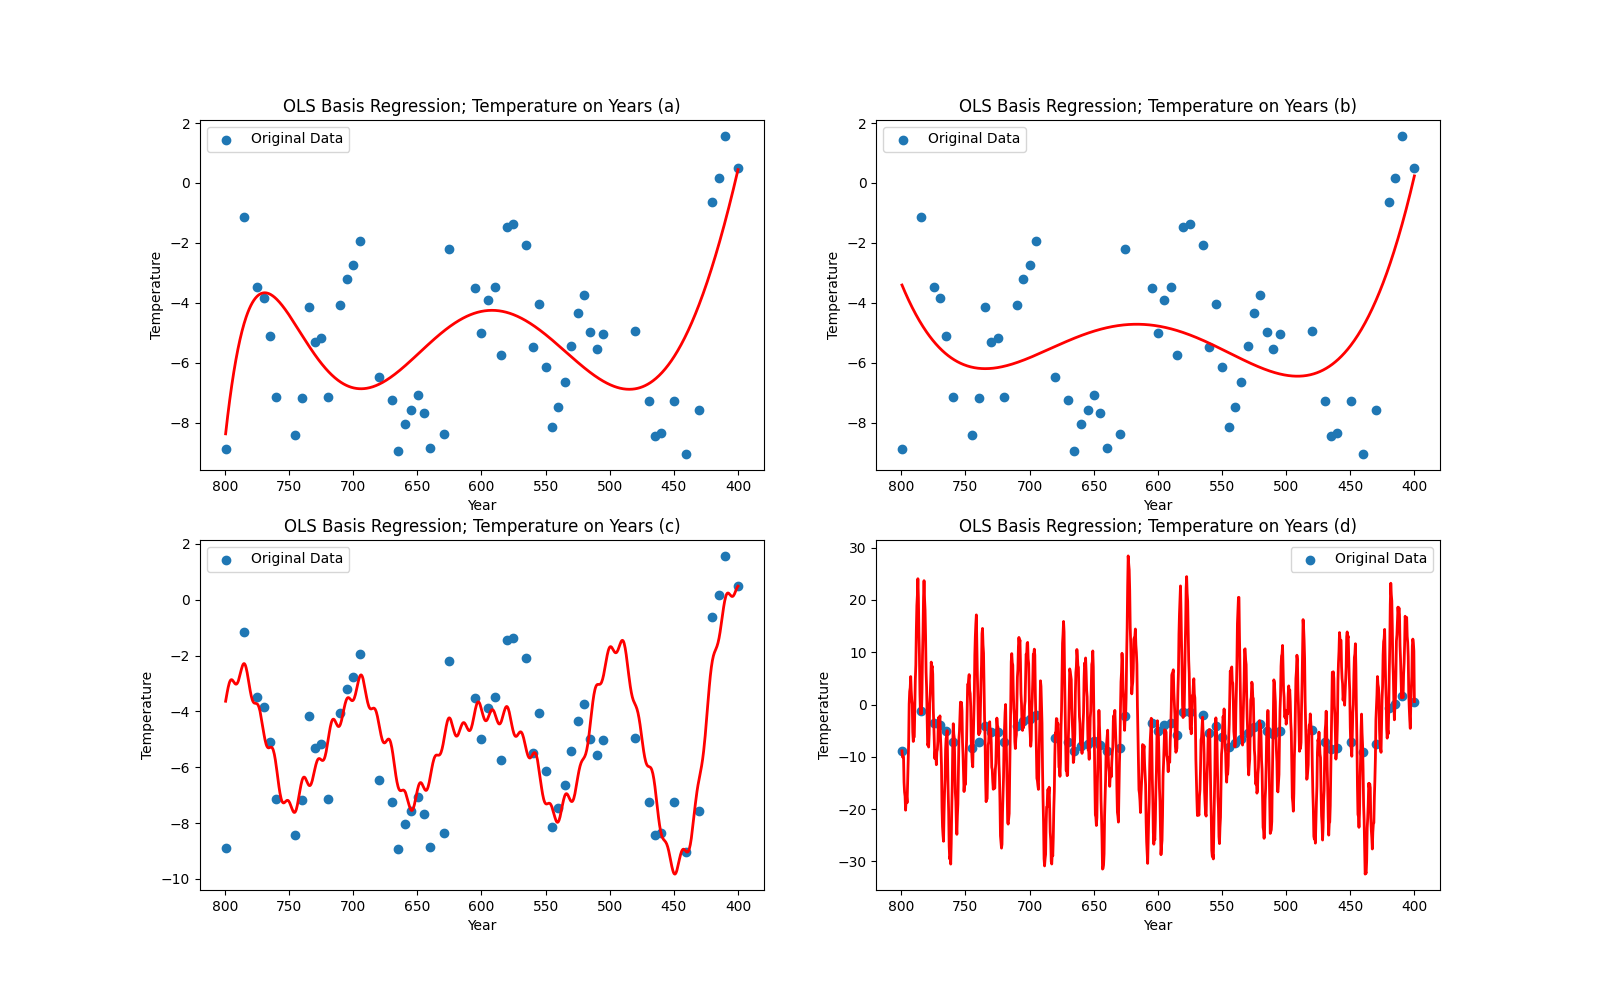
\includegraphics[width=0.8\textwidth]{img_output/p3.1.png}
  
    \item 
    Well, the MSE for the first three models is relatively similar to each other. Model number one seems to have a decent fit to the data. Model two is pretty underfit to the data. Model three is relatively well fit to the data. 
    

    It's obvious that the fourth model underfits the data because the test MSE is so high.
    
  
    \item 
  
    The purpose of the F transforms is to map the data, which is not necessarily linear, into a space that is linear so that we can apply the properties of linear regression.
    this allows us to use the very powerful tool of linear regression in a case where we normally would not be able to. One of the key assumptions of linear regression is that the data must be linear. This is extremely restrictive; using F transforms allows us to use this power, simple, and interpretable model. 

  
    \item 
    
    The space complexity of lienar regression is $O(ND)$ because we need to store N data points and D features. \newline 
    Since X is a matrix of size N x w, finding $(X' X)$ is $O(Nw^2)$ and finding the inverse is $O(w^3)$ \newline
    $(X' Y)$ takes$ O(n*w^2)$ time and gives us a $ w x w $ matrix \newline
    finally the matrix multiplication takes $O(w^3)$ time \newline
    so the overall time is $O(w^2*(n + w))$ 
    \newline

    The storage does not change with the size of the training set N; we only need to store the calucated coefficeints for the features w. So we only need to store w numbers.  \newline
    The time to compute also does not change based onthe training size--the computation only relies on the final parameters w -- we are calcualting the dot product of $ y = w^Tx$ \newline

    kNN \newline
    Storage complexity is $O(N)$ because we need to store N data points. \newline
    Time complexity is $O(Nw)$ or maybe $O(N log(w))$ because we need to find the k nearest neighbors -- the distance formula is the complex part. \newline


    Kernelized regression \newline
    Storage complexity is $O(N)$ because we need to store N data points. \newline
    Prediction time we need to calculate the kernel for all of the points to each of hte other points. If the kernel function is $O(w)$, then the time complexity is $O(N*w)$ \newline

    \item 
    We have three different kinds of regressors. \newline

    I don't think there is an objective "best" and "worst", but each is definetley situational and only applicable in certain cases. \newline

    kNN is certainly limited in the sense that it is not able to extrapolate. It can only predict based on the data it has seen. \newline

    Kernelized regression is a bit more flexible because it is able to use a kernel(a weighting function to determine different distances) but it is still limited in the sense that it is not able to extrapolate. It can only predict based on the data it has seen. \newline

    Linear regression is able to extrapolate, but it is a parametric model and the data may need to be massaged (transformed) into being linear to fit the assumptions. There are quite a few assumptions for lienar regression which makes it a little less flexible. 



    \end{enumerate}

  \end{tcolorbox}





\end{solution}

%%%%%%%%%%%%%%%%%%%%%%%%%%%%%%%%%%%%%%%%%%%%%
% Problem 4
%%%%%%%%%%%%%%%%%%%%%%%%%%%%%%%%%%%%%%%%%%%%%
\begin{problem}[Probablistic Regression and Regularization, 30pts]

Finally, we will preview Bayesian regression and explore its connection to regularization for linear models. Then, we will fit a regularized model to the temperature data. Although the content is related, you do not need to know the material from the lectures on frequentist model selection and Bayesian model selection to solve this problem.  \\

\noindent Recall that the probabilistic version of linear regression states that 
\[y_n = \boldw^\top\boldx_n + \epsilon_n, \quad \epsilon_n \sim \mathcal{N}(0, \sigma^2)\]
In Bayesian regression, we impose a prior $p(\boldw)$ on the weights and  fit the weights $\boldw$ through maximizing the posterior likelihood
\[p(\boldw | \boldX, \boldy) = \frac{p(\bold y | \boldw, \boldX)p(\boldw)}{p(\boldy | \boldX)}\]
Note: since we maximize with respect to $\boldw$, it suffices to just maximize the numerator.

\begin{enumerate}
    \item Suppose $\boldw \sim \mathcal{N}(\mathbf{0},\frac{\sigma^2}{\lambda}\boldI)$. Show that maximizing the posterior likelihood is equivalent to minimizing 
    \[\mathcal{L}_{ridge}(\boldw) = \frac{1}{2}||\boldy -\bold X\boldw||_2^2 + \frac{\lambda}{2}||\boldw||_2^2.\] 
    Note that minimizing $\mathcal{L}_{ridge}(\boldw)$ is exactly what ridge regression does.
    
    Hint: You don't need to solve for the maximizer/minimizer to show that the optimization problems are equivalent.
    
    \item Solve for the value of $\boldw$ that minimizes $\mathcal L_{ridge}(\boldw)$.

    \item The Laplace distribution has the PDF
   \[L(a,b) =\frac{1}{2b} \exp\left(-\frac{|x - a|}{b}\right)\]
Show that if all $w_d \sim L\left(0,\frac{2\sigma^2}{\lambda}\right)$, maximizing the posterior likelihood is equivalent to minimizing 
\[\mathcal{L}_{lasso}(\boldw) = \frac{1}{2}||\boldy -\bold X\boldw||_2^2  + \frac{\lambda}{2}||\boldw||_1.\] 
Note that minimizing $\mathcal{L}_{lasso}(\boldw)$ is exactly what LASSO regression does.

    \item Why is there no general closed form for the LASSO estimator, i.e. the value of $\boldw$ that minimizes $\mathcal{L}_{ridge}(\boldw)$?

    \item Since there is no general closed form for LASSO, we use numerical methods for estimating $\boldw$. One approach is to use \textit{coordinate descent}, which works as follows: 
    \begin{enumerate}
        \item Initialize $\boldw=\boldw_0$.
        \item For each $d=1, \ldots, D$ do the following 2 steps consecutively:
        \begin{enumerate}
            \item Compute $\rho_d = \tilde{\boldx}_d^\top(\boldy - (\boldX \boldw - w_d \tilde{\boldx}_d))$. We define $\tilde{\boldx}_d$ as the $d$-th column of $\boldX$.

            \item If $d=1$, set $w_1 = \frac{\rho_1}{||\tilde{\boldx}_1||^2_2}$. Otherwise if $d\ne 1$, compute $w_d = \frac{\text{sign}(\rho_d)\max\left\{|\rho_d|-\frac{\lambda}{2}, 0\right\}}{||\tilde{\boldx}_d||^2_2}$.
        \end{enumerate}
        \item Repeat step (b) until convergence or the maximum number of iterations is reached.
    \end{enumerate} 

    Implement the \texttt{find\_lasso\_weights} function according to the above algorithm, letting $\boldw_0$ be a vector of ones and the max number of iterations be 5000. Then, fit models with $\lambda=1, 10$ to basis (d) from Problem 3, plot the predictions, and compute the MSE's. You will need to do some preprocessing, but a completed helper function for this is already provided. How do the graphs and errors compare to those for the unregularized basis (d) model? 


\end{enumerate}

\end{problem}

\newpage
\begin{tcolorbox}[title=Solution, colback=white, colframe=black, breakable]
  \begin{enumerate}
      \item 
      
      First, we need to write out the likelihood function:

\[
y_n = \hat{\omega}^T x_n + \epsilon_n \quad \text{where} \quad \epsilon_n \sim \mathcal{N}(0, \sigma^2)
\]

Thus,

\[
\hat{y}_n | \hat{\omega} \sim \mathcal{N}(\hat{X} \hat{\omega}, \sigma^2 I)
\]

\[
P(\hat{y}_n | \hat{\omega}) = \left( \frac{1}{\sqrt{(2\pi \sigma^2)^N}} \right) \exp \left( -\frac{1}{2\sigma^2} \|\hat{y} - \hat{X} \hat{\omega} \|_2^2 \right)
\]

We have a prior for \( \hat{\omega} \):

\[
\hat{\omega} \sim \mathcal{N} (\hat{0}, \frac{\sigma^2}{\lambda} I)
\]

\[
P(\hat{\omega}) = \left( \frac{1}{\sqrt{(2\pi \frac{\sigma^2}{\lambda})^D}} \right) \exp \left( -\frac{\lambda}{2\sigma^2} \|\hat{\omega} \|_2^2 \right)
\]

\section*{Find the Posterior}

\[
P(\hat{\omega} | \hat{X}, \hat{y}) \propto \exp \left[ -\frac{1}{2\sigma^2} \left( \|\hat{y} - \hat{X} \hat{\omega} \|_2^2 + \lambda \|\hat{\omega} \|_2^2 \right) \right]
\]

Finding the Maximum A Posteriori is the same as minimizing the negative log-posterior:

\[
-\log \left[ P(\hat{\omega} | \hat{X}, \hat{y}) \right] \propto \frac{1}{2\sigma^2} \left[ \|\hat{y} - \hat{X} \hat{\omega} \|_2^2 + \lambda \|\hat{\omega} \|_2^2 \right]
\]

Dropping the multiplicative constant:

\[
\propto \|\hat{y} - \hat{X} \hat{\omega} \|_2^2 + \lambda \|\hat{\omega} \|_2^2
\]

Dividing both sides by 2:

\[
\frac{1}{2} \|\hat{y} - \hat{X} \hat{\omega} \|_2^2 + \frac{\lambda}{2} \|\hat{\omega} \|_2^2
\]

which is exactly the ridge regression loss function.

MAP is equal to min ridge.




      \item 
      
      Solving for \( \mathbf{\hat{w}} \) which minimizes \( L_{\text{ridge}} (\mathbf{w}) \).

Take derivative of result from 1:

\[
\frac{dL_{\text{ridge}} (\mathbf{w})}{d\mathbf{w}}
\]

\[
L_{\text{ridge}} (\mathbf{w}) = \frac{1}{2} (\mathbf{y} - X\mathbf{w})^T (\mathbf{y} - X\mathbf{w}) + \frac{\lambda}{2} \mathbf{w}^T \mathbf{w}
\]

Derivative of the first term:

\[
\nabla_{\mathbf{w}} f(\mathbf{w}) = -X^T (\mathbf{y} - X\mathbf{w})
\]

by the chain rule.

Derivative of the second term:

\[
\nabla_{\mathbf{w}} \left( \frac{\lambda}{2} \mathbf{w}^T \mathbf{w} \right) = \lambda \mathbf{w}
\]

Thus,

\[
\nabla_{\mathbf{w}} L_{\text{ridge}} (\mathbf{w}) = -X^T (\mathbf{y} - X\mathbf{w}) + \lambda \mathbf{w}
\]

Rearrange:

\[
\nabla_{\mathbf{w}} L_{\text{ridge}} (\mathbf{w}) = X^T X \mathbf{w} - X^T \mathbf{y} + \lambda \mathbf{w}
\]

Set equal to 0 and solve for \( \mathbf{w} \):

\[
X^T \mathbf{y} = (X^T X + \lambda I) \mathbf{w}
\]

Assume \( X^T X + \lambda I \) is invertible, multiply both sides by its inverse to get:

\[
\mathbf{\hat{w}} = (X^T X + \lambda I)^{-1} X^T \mathbf{y}
\]





      \item 
      
      This is a very similar process to part 1 of this question. We will use the same setups before:

      \[
      P(\hat{y}_n | \hat{w}) = \left( \frac{1}{\sqrt{(2\pi \sigma^2)^N}} \right) \exp \left( \frac{-1}{2\sigma^2} \| \hat{y} - X\hat{w} \|_2^2 \right)
      \]
      
      However, now our prior is different:
      
      \[
      P(\hat{w}) = \frac{\lambda}{\sigma^2} \exp \left( \frac{-|\hat{w}|}{2\sigma^2 / \lambda} \right)
      \]
      
      Now,
      
      \[
      P(\hat{w} | X, \hat{y}) \propto \left( \frac{1}{\sqrt{(2\pi \sigma^2)^N}} \right) \exp \left( \frac{-1}{2\sigma^2} \| \hat{y} - X\hat{w} \|_2^2 \right)
      \]
      
      \[
      \frac{\lambda}{\sigma^2} \exp \left( \frac{-|\hat{w}|}{2\sigma^2 / \lambda} \right)
      \]
      
      Taking the negative log of this and dropping multiplicative constants:
      
      \[
      -\log P(\hat{w} | X, \hat{y}) \propto
      \]
      
      \[
      \left( \frac{1}{2\sigma^2} \| \hat{y} - X\hat{w} \|_2^2 \right) + \frac{\lambda |\hat{w}|}{2\sigma^2 / \lambda}
      \]
      
      Rearranging and dropping the \(\sigma^2\) constant,
      
      \[
      \propto \frac{1}{2} \| \hat{y} - X\hat{w} \|_2^2 + \frac{\lambda}{2} \| \hat{w} \|_1
      \]
      
      Thus, they are equivalent.



      \item There is no general closed form for LASSO because it is a non differentiable function. It contains an absolute value term which is not differentiable at 0. Thus, we must use other methods to solve for it.
      \item 
      \begin{lstlisting}[language=Python]
  def find_lasso_weights(lam, X, y):
      """
      Fit the weights of a LASSO linear regression through the coordinate descent algorithm.
      
      :param lam: the lambda parameter
      :param X: the design matrix with training set features (with first column as intercept)
      :param y: the training set labels
      :return: the fitted weights as a numpy array
      """
      n, d = X.shape
      w = np.ones(d)
      max_iter = 5000
      tol = 1e-6  # convergence tolerance
      
      col_norm_sq = np.sum(X**2, axis=0)
      
      for iteration in range(max_iter):
          w_old = w.copy()
          for j in range(d):
              # r_j = y - (Xw - w[j]*X[:, j])
              r_j = y - (X.dot(w) - w[j] * X[:, j])
              # rho_j = x_j^T r_j
              rho_j = np.dot(X[:, j], r_j)
              
              if j == 0:
                  w[j] = rho_j / col_norm_sq[j]
              else:
                  w[j] = np.sign(rho_j) * max(np.abs(rho_j) - lam/2, 0) / col_norm_sq[j]
          
          # convergence check
          if np.max(np.abs(w - w_old)) < tol:
              break
              
      return w
      \end{lstlisting}
  
      \begin{lstlisting}[language=Python]
  # Helper function for standardizing inputs to LASSO
  def preprocess_lasso(X):
      X = make_basis(X, part='d')
      X[:, 1:] = (X[:, 1:] - X[:, 1:].mean(axis=0)) / X[:, 1:].std(axis=0)
      return X
      \end{lstlisting}
  
      \begin{lstlisting}[language=Python]
  # Fit the weights for both models
  phi_x_train = preprocess_lasso(year_train)
  
  lam1, lam2 = 1, 10
  
  w1 = find_lasso_weights(lam1, phi_x_train, temp_train)
  w2 = find_lasso_weights(lam2, phi_x_train, temp_train)
  
  x_array = np.arange(400, 801)
  phi_x_array = preprocess_lasso(x_array)
  
  y_pred1 = phi_x_array.dot(w1)
  y_pred2 = phi_x_array.dot(w2)
  
  plt.figure(figsize=(10, 6))
  plt.plot(x_array, y_pred1, label=f'LASSO (lambda = {lam1})', color='blue')
  plt.plot(x_array, y_pred2, label=f'LASSO (lambda = {lam2})', color='green')
  plt.scatter(year_train, temp_train, label="Training Data", color="red")
  plt.xlabel("Year BCE (in thousands)")
  plt.ylabel("Temperature")
  plt.title("LASSO Regression using Coordinate Descent")
  plt.xticks(np.arange(400, 901, 100))
  plt.gca().invert_xaxis()
  plt.legend()
  plt.savefig("img_output/p4.5.png", bbox_inches="tight")
  plt.show()
      \end{lstlisting}
  
      \begin{lstlisting}[language=Python]
  y_train_pred1 = phi_x_train.dot(w1)
  y_train_pred2 = phi_x_train.dot(w2)
  mse1 = np.mean((temp_train - y_train_pred1)**2)
  mse2 = np.mean((temp_train - y_train_pred2)**2)
  
  print("MSE for LASSO with lambda = 1:", mse1)
  print("MSE for LASSO with lambda = 10:", mse2)
      \end{lstlisting}


    FINAL ANSWER FOR PART 5: \newline

 

    MSE for LASSO with lambda = 1: 1.9508996956712439 \newline
    MSE for LASSO with lambda = 10: 3.136512716950103

    Clearly, at a point, using LASSO with too high a lambda will degrade the quality of the model. We are essentially "overcorrecting" the fit of the data. As lambda is a hyperparameter, we would want to find an idealized lambda value which minimizes the validation / test MSE

  
  \end{enumerate}
  \end{tcolorbox}
  \begin{figure}[h]
    \centering
    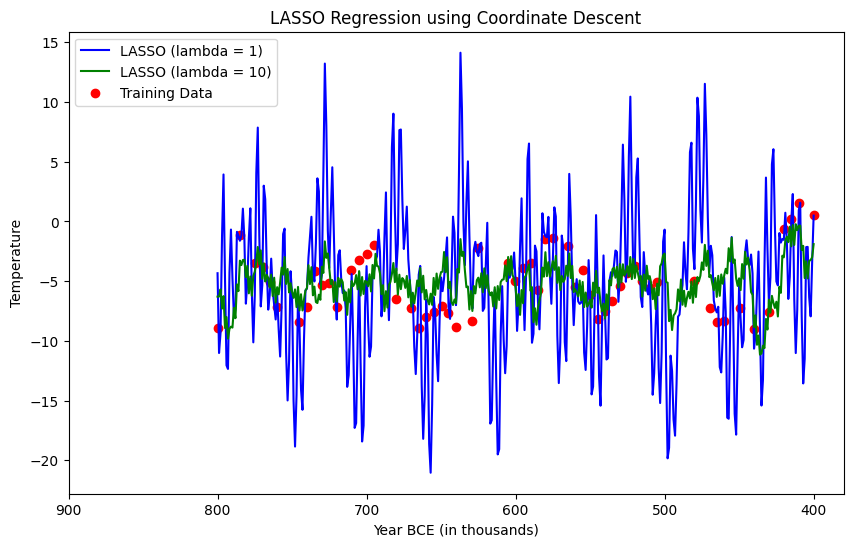
\includegraphics[width=0.75\textwidth]{img_output/p4.5.png}
    \caption{LASSO regression predictions using coordinate descent with $\lambda=1$ and $\lambda=10$.}
  \end{figure}



%%%%%%%%%%%%%%%%%%%%%%%%%%%%%%%%%%%%%%%%%%%%%
% Name and Calibration
%%%%%%%%%%%%%%%%%%%%%%%%%%%%%%%%%%%%%%%%%%%%%
\newpage
\subsection*{Matt Krasnow}

\subsection*{Collaborators and Resources}
Whom did you work with, and did you use any resources beyond cs181-textbook and your notes?

I worked with me myself and I because im cool


\end{document}
